\documentclass[compress,color=usenames]{beamer}

\newcommand{\mytitlenbr}{1}
\newcommand{\mytitle}{Image Archive}

%\documentclass[compress,color=usenames,handout]{beamer}

%\usepackage{pgfpages}
%\pgfpagelayout{4 on 2}[a4paper,border shrink=5mm]

\usepackage{graphicx}
\usepackage{amsfonts,amssymb}
\usepackage{latexsym}
\usepackage{mdwtab}
\usepackage{xspace}

\DefineNamedColor{named}{Periwinkle}{cmyk}{0.57,0.55,0,0}
\DefineNamedColor{named}{Plum}{cmyk}{0.50,1,0,0}
\DefineNamedColor{named}{Red}{cmyk}{0,1,1,0}

\newcommand{\mH}[1]{\textcolor{Plum}{#1}}
\newcommand{\mT}[1]{\textcolor{Periwinkle}{#1}}

\newcommand{\tup}[1]{\langle #1 \rangle}

\newcommand{\dd}{{:}}
\newcommand{\I}{\mathcal{I}}
\newcommand{\csetsc}[2]{\{#1 \mid #2\}}
\newcommand{\cset}[1]{\{#1\}}

\newcommand{\CON}{\textsf{CON}\xspace}
\newcommand{\ROL}{\textsf{ROL}\xspace}
\newcommand{\IND}{\textsf{IND}\xspace}
\newcommand{\PROP}{\textsf{PROP}\xspace}
\newcommand{\lang}{\mathcal{L}\xspace}


\newcommand{\mytt}[1]{\textsf{\scriptsize{#1}}}
\newcommand{\mytts}[1]{\textsf{\scriptsize{#1}}}

%\usefonttheme{serif}

\mode<presentation>
 {
 \usetheme{lined}
 }

\setbeamertemplate{navigation symbols}{}


\newcommand{\F}{\mathop{\mathsf{F}\vphantom{a}}\nolimits}
\newcommand{\G}{\mathop{\mathsf{G}\vphantom{a}}\nolimits}
\newcommand{\X}{\mathop{\mathsf{X}\vphantom{a}}\nolimits}

\newcommand{\Blue}[1]{\textcolor{blue}{#1}}
\newcommand{\Red}[1]{\textcolor{red}{#1}}
\newcommand{\Green}[1]{\textcolor{PineGreen}{#1}}


\title[GLN y Aplicaciones]{\Huge Generaci\'on de Lenguaje Natural y Aplicaciones}
%\mH{Lecture \#\mytitlenbr:} \mytitle}

\author[Areces \& Benotti]{
 Carlos Areces y Luciana Benotti\\[1ex]
\normalsize \url{{carlos.areces, luciana.benotti}@gmail.com}}

\institute[INRIA / UNC]{
INRIA Nancy Grand Est, Nancy, France\\
Universidad Nacional de C\'ordoba, C\'ordoba, Argentina}

\date{ELiC 2010 - Buenos Aires - Argentina}

\begin{document}


\beamerdefaultoverlayspecification{}


\begin{frame}[plain]
 \titlepage
\end{frame}

\begin{frame}
\frametitle{What This Tutorial is About}

\label{f0}
\begin{itemize}
\item { {The design and construction of systems which}}
\begin{itemize}
\item produce understandable texts in English or other human languages ...
\item from some underlying non-linguistic representation of information 
\item using knowledge about language and the application domain.
\end{itemize}
\item { {Based on:}}
\item { { E Reiter and R Dale \mbox{$[$}1999\mbox{$]$} \textit{Building Natural Language Generation Systems}. Cambridge University Press.}}
\end{itemize}

\end{frame}

\begin{frame}
\frametitle{Goals of the Tutorial}

\label{f2}
\begin{itemize}
\item { {For managers:}}
\begin{itemize}
\item to provide a broad overview of the field and what is possible today
\end{itemize}
\item { {For implementers:}}
\begin{itemize}
\item to provide a realistic assessment of available techniques
\end{itemize}
\item { {For researchers:}}
\begin{itemize}
\item to highlight the issues that are important in current applied NLG projects
\end{itemize}
\end{itemize}



\end{frame}

\begin{frame}
\frametitle{Overview}

\label{f6}
\begin{itemize}
\item { {1 An Introduction to NLG}}
\item { {2 Requirements Analysis and a Case Study}}
\item { {3 The Component Tasks in NLG}}
\item { {4 NLG in Multimedia and Multimodal Systems}}
\item { {5 Conclusions and Pointers}}
\end{itemize}


\end{frame}

\begin{frame}
\frametitle{An Introduction to NLG}

\label{f8}
\begin{itemize}
\item { {What is Natural Language Generation?}}
\item { {Some Example Systems}}
\item { {Types of NLG Applications}}
\item { {When are NLG Techniques Appropriate?}}
\item { {NLG System Architecture}}
\end{itemize}


\end{frame}

\begin{frame}
\frametitle{What is NLG?}

\label{f10}
\begin{itemize}
\item { {Natural language generation is the process of deliberately constructing a natural language text in order to meet specified communicative goals.}}\\

\hfill [McDonald 1992]
\end{itemize}


\end{frame}

\begin{frame}
\frametitle{What is NLG?}

\label{f12}
\begin{itemize}
\item { {Goal: }}
\begin{itemize}
\item computer software which produces understandable and appropriate texts in English or other human languages
\end{itemize}
\item { {Input: }}
\begin{itemize}
\item some underlying non-linguistic representation of information
\end{itemize}
\item { {Output: }}
\begin{itemize}
\item documents, reports, explanations, help messages, and other kinds of texts
\end{itemize}
\item { {Knowledge sources required: }}
\begin{itemize}
\item knowledge of language and of the domain
\end{itemize}
\end{itemize}

\end{frame}

\begin{frame}
\frametitle{Language Technology}

\begin{center}
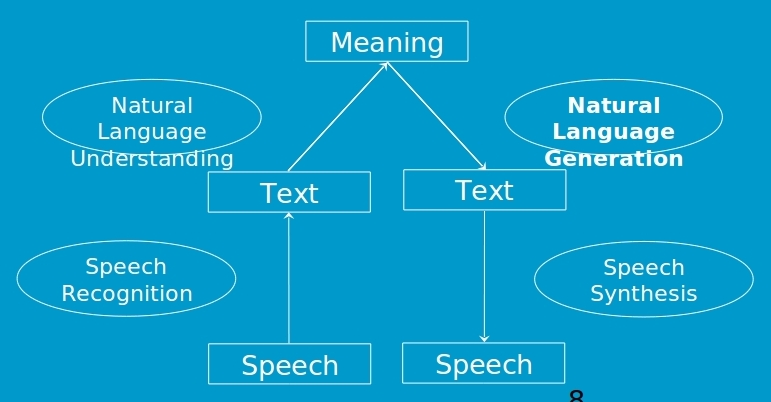
\includegraphics[scale=.3]{pics/pic1.jpg}
\end{center}
\end{frame}

\begin{frame}
\frametitle{Example System \#1: FoG}

\label{f16}
\begin{itemize}
\item { {Function: }}
\begin{itemize}
\item Produces textual weather reports in English and French 
\end{itemize}
\item { {Input: }}
\begin{itemize}
\item Graphical/numerical weather depiction
\end{itemize}
\item { {User: }}
\begin{itemize}
\item Environment Canada (Canadian Weather Service)
\end{itemize}
\item { {Developer: }}
\begin{itemize}
\item CoGenTex
\end{itemize}
\item { {Status: }}
\begin{itemize}
\item Fielded, in operational use since 1992
\end{itemize}
\end{itemize}
\end{frame}

\begin{frame}
\frametitle{FoG: Input}

\begin{center}
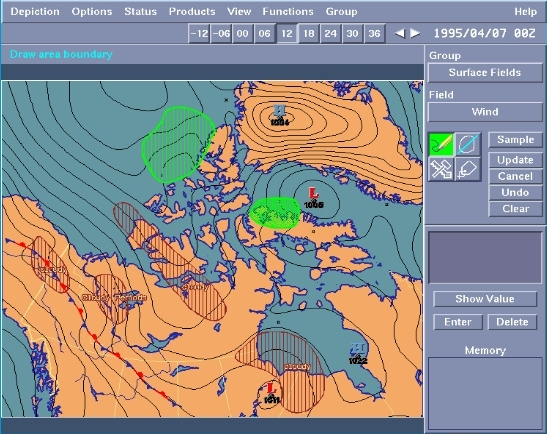
\includegraphics[scale=.4]{pics/pic2.jpg}
\end{center}

\end{frame}

\begin{frame}
\frametitle{FoG: Output}

\begin{center}
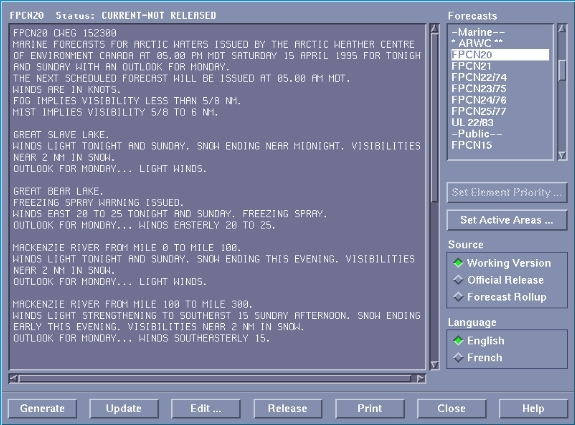
\includegraphics[scale=.4]{pics/pic3.jpg}
\end{center}

\end{frame}

\begin{frame}
\frametitle{Example System \#2: PlanDoc}

\label{f22}
\begin{itemize}
\item { {Function: }}
\begin{itemize}
\item Produces a report describing the simulation options that an engineer has explored
\end{itemize}
\item { {Input: }}
\begin{itemize}
\item A simulation log file
\end{itemize}
\item { {User: }}
\begin{itemize}
\item Southwestern Bell
\end{itemize}
\item { {Developer: }}
\begin{itemize}
\item Bellcore and Columbia University
\end{itemize}
\item { {Status: }}
\begin{itemize}
\item Fielded, in operational use since 1996
\end{itemize}
\end{itemize}

\end{frame}

\begin{frame}
\frametitle{PlanDoc: Input}

\label{f24}
\begin{itemize}
\item { {RUNID fiberall FIBER 6/19/93 act yes}}
\item { {FA 1301 2 1995}}
\item { {FA 1201 2 1995}}
\item { {FA 1401 2 1995}}
\item { {FA 1501 2 1995}}
\item { {ANF co 1103 2 1995 48}}
\item { {ANF 1201 1301 2 1995 24}}
\item { {ANF 1401 1501 2 1995 24}}
\item { {END. 856.0 670.2}}
\end{itemize}

\end{frame}

\begin{frame}
\frametitle{PlanDoc: Output}

\label{f26}
\begin{itemize}
\item { {This saved fiber refinement includes all DLC changes in Run-ID ALLDLC. RUN-ID FIBERALL demanded that PLAN activate fiber for CSAs 1201, 1301, 1401 and 1501 in 1995 Q2. It requested the placement of a 48-fiber cable from the CO to section 1103 and the placement of 24-fiber cables from section 1201 to section 1301 and from section 1401 to section 1501 in the second quarter of 1995. For this refinement, the resulting 20 year route PWE was \$856.00K, a \$64.11K savings over the BASE plan and the resulting 5 year IFC was \$670.20K, a \$60.55K savings over the BASE plan.}}
\end{itemize}

\end{frame}

\begin{frame}
\frametitle{Example System \#3: STOP}

\label{f28}
\begin{itemize}
\item { {Function: }}
\begin{itemize}
\item Produces a personalised smoking-cessation leaflet
\end{itemize}
\item { {Input: }}
\begin{itemize}
\item Questionnaire about smoking attitudes, beliefs, history
\end{itemize}
\item { {User: }}
\begin{itemize}
\item NHS (British Health Service)
\end{itemize}
\item { {Developer: }}
\begin{itemize}
\item University of Aberdeen 
\end{itemize}
\item { {Status: }}
\begin{itemize}
\item Undergoing clinical evaluation to determine its effectiveness
\end{itemize}
\end{itemize}

\end{frame}

\begin{frame}
\frametitle{STOP: Input}

\begin{center}
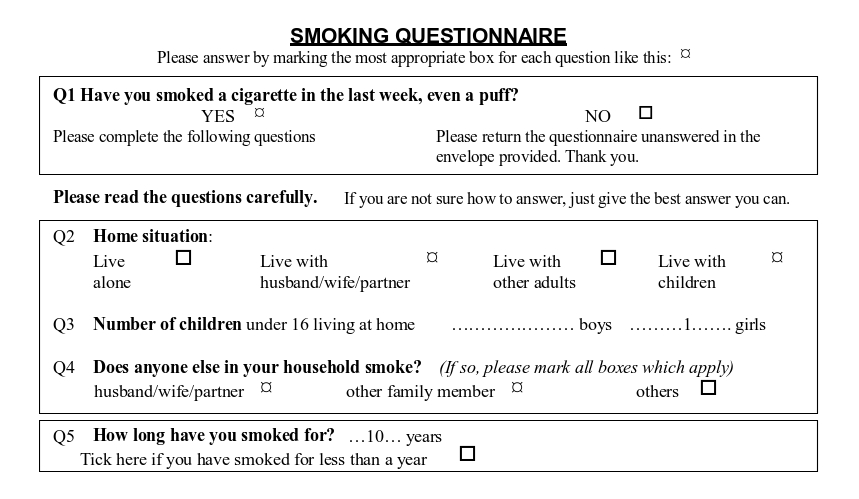
\includegraphics[scale=.4]{pics/pic4.jpg}
\end{center}

\end{frame}

\begin{frame}
\frametitle{STOP: Output}

 { {{Dear Ms Cameron}}}

 { {Thank you for taking the trouble to return the smoking questionnaire that we sent you. It appears from your answers that although you're not planning to stop smoking in the near future, you would like to stop if it was easy. You think it would be difficult to stop because \textit{smoking helps you cope with stress, it is something to do when you are bored, and smoking stops you putting on weight}. However, you have reasons to be confident of success if you did try to stop, and there are ways of coping with the difficulties. }}

\end{frame}

\begin{frame}
\frametitle{Example System \#4: TEMSIS}

\label{f34}
\begin{itemize}
\item { {Function: }}
\begin{itemize}
\item Summarises pollutant information for environmental officials
\end{itemize}
\item { {Input: }}
\begin{itemize}
\item Environmental data + a specific query
\end{itemize}
\item { {User: }}
\begin{itemize}
\item Regional environmental agencies in France and Germany
\end{itemize}
\item { {Developer: }}
\begin{itemize}
\item DFKI GmbH
\end{itemize}
\item { {Status: }}
\begin{itemize}
\item Prototype developed; requirements for fielded system being analysed
\end{itemize}
\end{itemize}

\end{frame}

\begin{frame}[fragile]
\frametitle{TEMSIS: Input Query}

\begin{verbatim}
((LANGUAGE FRENCH)
  (GRENZWERTLAND GERMANY)
  (BESTAETIGE-MS T)
  (BESTAETIGE-SS T) 
  (MESSSTATION \"Voelklingen City\"
  (DB-ID \"#2083\"
  (SCHADSTOFF \"#19\"
  (ART MAXIMUM)
  (ZEIT ((JAHR 1998)
         (MONAT 7)
         (TAG 21))))
\end{verbatim}


\end{frame}

\begin{frame}
\frametitle{TEMSIS: Output Summary}

\begin{itemize}
\item Le 21/7/1998 \`a la station de mesure de V\"olklingen-City, la valeur moyenne maximale d'une demi-heure (Halbstundenmittelwert) pour l'ozone atteignait 104.0 $\mu$g/m${}^3$. Par cons\'equent, selon le decret MIK (MIK-Verordnung), la valeur limite autoris\'ee de 120 $\mu$g/m${}^3$ n'a pas \'et\'e d\'epass\'e.

\item Der h\"ochste Halbstundenmittelwert f\"ur Ozon an der Me{\ss}station V\"olklingen-City erreichte 
am 21.7.1998 104.0 $\mu$g/m${}^3$, womit der gesetzlich zul\"assige Grenzwert nach MIK-Verordnung von 
120 $\mu$g/m${}^3$ nicht \"uberschritten wurde.
\end{itemize}

\end{frame}

\begin{frame}
\frametitle{Types of NLG Applications}

\label{f40}
\begin{itemize}
\item { {Automated document production}}
\begin{itemize}
\item weather forecasts, simulation reports, letters, ...
\end{itemize}
\item { {Presentation of information to people in an understandable fashion}}
\begin{itemize}
\item medical records, expert system reasoning, ...
\end{itemize}
\item { {Teaching}}
\begin{itemize}
\item information for students in CAL systems
\end{itemize}
\item { {Entertainment}}
\begin{itemize}
\item jokes (?), stories (??), poetry (???)
\end{itemize}
\end{itemize}

\end{frame}

\begin{frame}
\frametitle{The Computer\^as Role}

\label{f42}
\begin{itemize}
\item { {Two possibilities:}}
\item { {\#1 The system produces a document without human help: }}
\item { {weather forecasts, simulation reports, patient letters}}
\item { {summaries of statistical data, explanations of expert system reasoning, context-sensitive help, }}
\item { {\#2 The system helps a human author create a document:}}
\item { {weather forecasts, simulation reports, patient letters}}
\item { {customer-service letters, patent claims, technical documents, job descriptions, ...}}
\end{itemize}

\end{frame}

\begin{frame}
\frametitle{When are NLG Techniques Appropriate?}

\label{f44}
\begin{itemize}
\item { {Options to consider:}}
\item { {Text vs Graphics}}
\begin{itemize}
\item Which medium is better?
\end{itemize}
\item { {Computer generation vs Human authoring}}
\begin{itemize}
\item Is the necessary source data available?
\item Is automation economically justified?
\end{itemize}
\item { {NLG vs simple string concatenation}}
\begin{itemize}
\item How much variation occurs in output texts?
\item Are linguistic constraints and optimisations important?
\end{itemize}
\end{itemize}

\end{frame}

\begin{frame}
\frametitle{Enforcing Constraints}

\label{f46}
\begin{itemize}
\item { {Linguistically well-formed text involves many constraints:}}
\begin{itemize}
\item orthography, morphology, syntax
\item reference, word choice, pragmatics
\end{itemize}
\item { {Constraints are automatically enforced in NLG systems}}
\begin{itemize}
\item automatic, covers 100\% of cases
\end{itemize}
\item { {String-concatenation system developers must explicitly enforce constraints by careful design and testing}}
\begin{itemize}
\item A lot of work
\item Hard to guarantee 100\% satisfaction
\end{itemize}
\end{itemize}

\end{frame}

\begin{frame}
\frametitle{Example: Syntax, aggregation}

\label{f48}
\begin{itemize}
\item { {Output of existing Medical AI system:}}
\begin{itemize}
\item The primary measure you have chosen, CXR shadowing, should be justified in comparison to TLC and walking distance as my data reveals they are better overall. Here are the specific comparisons:
\item TLC has a lower patient cost TLC is more tightly distributed TLC is more objective walking distance has a lower patient cost
\end{itemize}
\end{itemize}

\end{frame}

\begin{frame}
\frametitle{Example: Pragmatics}

\label{f50}
\begin{itemize}
\item { {Output of system which gives English versions of database queries:}}
\begin{itemize}
\item The number of households such that there is at least 1 order with dollar amount greater than or equal to \$100.
\item Humans interpret this as number of \^ahouseholds which have placed an order \mbox{$>$}= \$100\^a
\item Actual query returns count of all households in DB if there is any order in the DB (from any household) which is \mbox{$>$}=\$100
\end{itemize}
\end{itemize}

\end{frame}

\begin{frame}
\frametitle{NLG System Architecture}

\label{f52}
\begin{itemize}
\item { {The Component Tasks in NLG}}
\item { {A Pipelined Architecture}}
\item { {Alternative Architectures}}
\end{itemize}

\end{frame}

\begin{frame}
\frametitle{Component Tasks in NLG}

\label{f54}
\begin{itemize}
\item { {1 Content determination}}
\item { {2 Document structuring}}
\item { {3 Aggregation}}
\item { {4 Lexicalisation}}
\item { {5 Referring expression generation}}
\item { {6 Linguistic realisation}}
\item { {7 Structure realisation}}
\end{itemize}

\end{frame}

\begin{frame}
\frametitle{Tasks and Architecture in NLG}

\begin{center}
\begin{tabular}{|l|c|}  \hline
Content Determination & Document \\
Document Structuring &  planning\\ \hline
Aggregation &  Micro-\\
Lexicalisation & planning\\
Referring Expression Generation & \\ \hline
Linguistic Realisation & Surface\\
Structure Realisation & realization\\ \hline
\end{tabular}
\end{center}

\end{frame}

\begin{frame}
\frametitle{A Pipelined Architecture}

\begin{center}
Document\\
planning\\
$\downarrow$\\
Document plan\\
$\downarrow$\\
Microplanning\\
$\downarrow$\\
Text Specificacion\\
$\downarrow$\\
Surface\\
Realization
\end{center}

\end{frame}

\begin{frame}
\frametitle{Other Architectures}

\label{f60}
\begin{itemize}
\item { {\#1: Variations on the \^astandard\^a architecture:}}
\item { {shift tasks around}}
\item { {allow feedback between stages}}
\item { {\#2: An integrated reasoner which does everything:}}
\item { {represent all tasks in the same way: eg as constraints, axioms, plan operators ...}}
\item { {feed specifications into a constraint-solver, theorem-prover ...}}
\end{itemize}

\end{frame}

\begin{frame}
\frametitle{Research Questions}

\label{f62}
\begin{itemize}
\item { {When is text the best means to communicate with the user?}}
\item { {When is NLG technology better than string concatenation?}}
\item { {Is there an architecture which combines the theoretical elegance of integrated approaches with the engineering simplicity of the pipeline?}}
\item { {How should document plans and text specifications be represented?}}
\end{itemize}

\end{frame}

\begin{frame}
\frametitle{Overview}

\label{f64}
\begin{itemize}
\item { {1 An Introduction to NLG}}
\item { {2 Requirements Analysis and a Case Study}}
\item { {3 The Component Tasks in NLG}}
\item { {4 NLG in Multimedia and Multimodal Systems}}
\item { {5 Conclusions and Pointers}}
\end{itemize}

\end{frame}

\begin{frame}
\frametitle{A Case Study in Applied NLG}

\begin{itemize}
\item { {Each month an institutional newsletter publishes a summary of the month's weather}}
\item { {The summaries are based on automatically collected meteorological data}}
\item { {The person who writes these summaries will no longer be able to}}
\item { {The institution wants to continue publishing the reports and so is interested in using NLG techniques to do so}}
\end{itemize}

\end{frame}

\begin{frame}
\frametitle{A Weather Summary}

\begin{center}
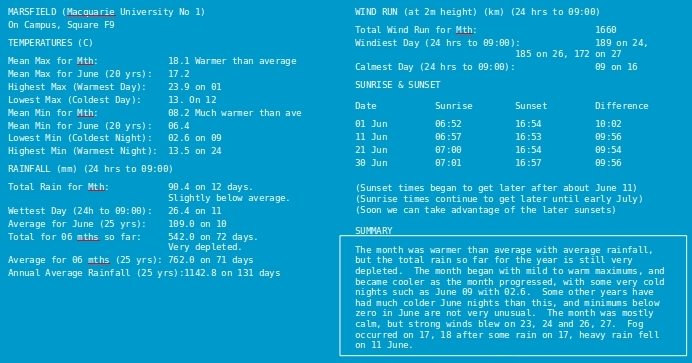
\includegraphics[scale=.47]{pics/pic5.jpg}
\end{center}

\end{frame}


\begin{frame}
\frametitle{Output: A Weather Summary}

\label{f70}
\begin{itemize}
\item { {The month was warmer than average with average rainfall, but the total rain so far for the year is still very depleted. The month began with mild to warm maximums, and became cooler as the month progressed, with some very cold nights such as June 09 with 02.6. Some other years have had much colder June nights than this, and minimums below zero in June are not very unusual. The month was mostly calm, but strong winds blew on 23, 24 and 26, 27. Fog occurred on 17, 18 after some rain on 17, heavy rain fell on 11 June.}}
\end{itemize}

\end{frame}

\begin{frame}[fragile]
\frametitle{The Input Data}

\begin{itemize}
\item { {A set of 16 data elements collected automatically every 15 minutes: air pressure, temperature, wind speed, rainfall }}
\item { {Preprocessed to construct DailyWeatherRecords:}}

\begin{verbatim}
((type dailyweatherrecord)
   (date ((day ...)
          (month ...)
          (year ...)))
 (temperature ((minimum ((unit degrees-centigrade)
                         (number ...)))
               (maximum ((unit degrees-centrigrade)
                         (number ...)))))
 (rainfall ((unit millimetres)
            (number ...))))
\end{verbatim}

\end{itemize}
\end{frame}

\begin{frame}
\frametitle{Other Available Data}

\label{f74}
\begin{itemize}
\item { {Historical Data: Average temperature and rainfall figures for each month in the Period of Record (1971 to present)}}
\item { {Historical Averages: Average values for temperature and rainfall for the twelve months of the year over the period of record}}
\end{itemize}

\end{frame}

\begin{frame}
\frametitle{Requirements Analysis}

\label{f76}
\begin{itemize}
\item { {The developer needs to:}}
\item { {understand the client\^as needs}}
\item { {propose a functionality which addresses these needs}}
\end{itemize}

\end{frame}

\begin{frame}
\frametitle{Corpus-Based Requirements Analysis}

\label{f78}
\begin{itemize}
\item { {A corpus:}}
\item { {consists of examples of output texts and corresponding input data}}
\item { {specifies \^aby example\^a the functionality of the proposed NLG system}}
\item { {is a very useful resource for design as well as requirements analysis}}
\end{itemize}

\end{frame}

\begin{frame}
\frametitle{Corpus-Based Requirements Analysis}

\label{f80}
\begin{itemize}
\item { {Four steps:}}
\item { {assemble an initial corpus of (human-authored) output texts and associated input data}}
\item { {analyse the information content of the corpus texts in terms of the input data}}
\item { {develop a target text corpus}}
\item { {create a formal functional specification}}
\end{itemize}

\end{frame}

\begin{frame}
\frametitle{Step 1: Creating an Initial Corpus}

\label{f82}
\begin{itemize}
\item { {Collect a corpus of input data and associated (human-authored) output texts}}
\item { {One source is archived examples of human-authored texts}}
\item { {If no human-authored examples of the required texts exist, ask domain experts to produce examples}}
\item { {The corpus should cover the full range of texts expected to be produced by the NLG system}}
\end{itemize}

\end{frame}

\begin{frame}
\frametitle{Initial Text (April 1995)}

\label{f84}
\begin{itemize}
\item { {SUMMARY}}
\item { {The month was rather dry with only three days of rain in the middle of the month. The total for the year so far is very depleted again, after almost catching up during March. Mars Creek dried up again on 30th April at the waterfall, but resumed on 1st May after light rain. This is the fourth time it dried up this year.}}
\end{itemize}

\end{frame}

\begin{frame}
\frametitle{Step 2: Analyzing the Content of the Texts}

\label{f86}
\begin{itemize}
\item { {Goal: }}
\begin{itemize}
\item to determine where the information present in the texts comes from, and the extent to which the proposed NLG system will have to manipulate this information
\end{itemize}
\item { {Result: }}
\begin{itemize}
\item a detailed understanding of the correspondences between the available input data and the output texts in the initial corpus
\end{itemize}
\end{itemize}


\end{frame}

\begin{frame}
\frametitle{Information Types in Text}

\label{f88}
\begin{itemize}
\item { {Unchanging text}}
\item { {Directly-available data}}
\item { {Computable data}}
\item { {Unavailable data}}
\end{itemize}

\end{frame}

\begin{frame}
\frametitle{Unchanging Text}

\mH{SUMMARY}

{ {The month was rather dry with only three days of rain in the middle of the month. The total for the year so far is very depleted again, after almost catching up during March. Mars Creek dried up again on 30th April at the waterfall, but resumed on 1st May after light rain. This is the fourth time it dried up this year.}}

\end{frame}

\begin{frame}
\frametitle{Directly Available Data}

SUMMARY

\mH{The month was rather dry with only three days of rain in the middle of the month}. The total for the year so far is very depleted again, after almost catching up during March. Mars Creek dried up again on 30th April at the waterfall, but resumed on 1st May after light rain. This is the fourth time it dried up this year.

\end{frame}

\begin{frame}
\frametitle{Computable Data}

SUMMARY

The month was rather dry with only three days of rain in the middle of the month. \mH{The total for the year so far is very depleted again, after almost catching up during March}. Mars Creek dried up again on 30th April at the waterfall, but resumed on 1st May after light rain. This is the fourth time it dried up this year.

\end{frame}

\begin{frame}
\frametitle{Unavailable Data}

SUMMARY

The month was rather dry with only three days of rain in the middle of the month. The total for the year so far is very depleted again, after almost catching up during March. \mH{Mars Creek dried up again on 30th April at the waterfall, but resumed on 1st May after light rain. This is the fourth time it dried up this year.}

\end{frame}


\begin{frame}
\frametitle{Solving the Problem of Unavailable Data}

\begin{itemize}
\item { {More information can be made available to the system: this may be expensive}}
    \begin{itemize}
        \item add sensors to Mars Creek?
    \end{itemize}
\item { {If the system is an authoring-aid, a human author can add this information}}
    \begin{itemize}
    \item system produces the first two sentences, the human adds the second two
    \end{itemize}
\item { {The target corpus can be revised to eliminate clauses that convey this information}}
    \begin{itemize}
    \item only produce the first two sentences
    \end{itemize}
\end{itemize}

\end{frame}

\begin{frame}
\frametitle{Step 3: Building theTarget Text Corpus}

\begin{itemize}
\item { {Mandatory changes:}}
\item { {eliminate unavailable data}}
\item { {specify what text portions will be human-authored}}
\item { {Optional changes:}}
\item { {simplify the text to make it easier to generate }}
\item { {improve human-authored texts}}
\item { {enforce consistency between human authors}}
\end{itemize}

\end{frame}

\begin{frame}
\frametitle{Target Text}

\begin{itemize}
\item { {The month was rather dry with only three days of rain in the middle of the month. The total for the year so far is very depleted again.}}
\end{itemize}

\end{frame}

\begin{frame}
\frametitle{Step 4: Functional Specification}

\label{f104}
\begin{itemize}
\item { {Based on an agreed target text corpus}}
\item { {Explicitly states role of human authoring, if present at all}}
\item { {Explicitly states structure and range of inputs to be used}}
\end{itemize}

\end{frame}

\begin{frame}
\frametitle{Initial Text \#2}

\label{f106}
\begin{itemize}
\item { {The month was our driest and warmest August in our 24 year record, and our first 'rainless' month. The 26th August was our warmest August day in our record with 30.1, and our first 'hot' August day (30). The month forms part of our longest dry spell 47 days from 18 July to 02 September 1995. Rainfall so far is the same as at the end of July but now is very deficient.}}
\end{itemize}

\end{frame}

\begin{frame}
\frametitle{Target Text \#2}

\label{f108}
\begin{itemize}
\item { {The month was the driest and warmest August in our 24 year record, and the first rainless month of the year. 26th August was the warmest August day in our record with 30.1, and the first hot day of the month. Rainfall for the year is now very deficient.}}
\end{itemize}

 \end{frame}

\begin{frame}
\frametitle{The Case Study So Far}

\label{f110}
\begin{itemize}
\item { {We\^all assume that:}}
\item { {We have located the source data}}
\item { {We have preprocessed the data to build the DailyWeatherRecords}}
\item { {We have constructed an initial corpus of texts}}
\item { {We have modified the initial corpus to produce a set of target texts}}
\end{itemize}

 \end{frame}


\begin{frame}
\frametitle{Is it Worth Using NLG?}

\label{f112}
\begin{itemize}
\item { {For one summary a month probably not, especially given the simplifications required to the texts to make them easy to generate}}
\item { {However, the client is interested in a pilot study: }}
\begin{itemize}
\item in the future there may be a shift to weekly summaries
\item there are many automatic weather data collection sites, each of which could use the technology
\end{itemize}
\end{itemize}

 \end{frame}

\begin{frame}
\frametitle{Research Issues}

\label{f114}
\begin{itemize}
\item { {Development of an appropriate corpus analysis methodology}}
\item { {Using expert system knowledge acquisition techniques}}
\item { {Automating aspects of corpus analysis}}
\item { {Integrating corpus analysis with standard requirements analysis procedures}}
\end{itemize}

 \end{frame}

\begin{frame}
\frametitle{Overview}

\label{f116}
\begin{itemize}
\item { {1 An Introduction to NLG}}
\item { {2 Requirements Analysis and a Case Study}}
\item { {3 The Component Tasks in NLG}}
\item { {4 NLG in Multimedia and Multimodal Systems}}
\item { {5 Conclusions and Pointers}}
\end{itemize}

 
\end{frame}

\begin{frame}
\frametitle{Inputs and Outputs}

\begin{center}
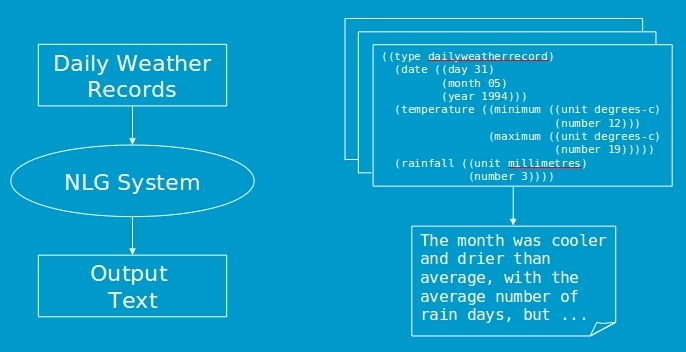
\includegraphics[scale=.3]{pics/pic6.jpg}
\end{center}

\end{frame}

\begin{frame}
\frametitle{The Architectural View}

\begin{center}
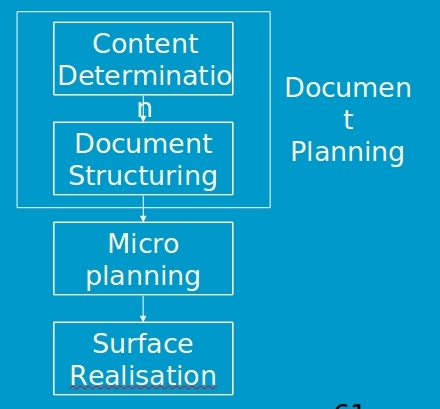
\includegraphics[scale=.3]{pics/pic7.jpg}
\end{center}
 
\end{frame}

\begin{frame}
\frametitle{Document Planning}

\label{f122}
\begin{itemize}
\item { {Goals: }}
\item { {to determine what information to communicate}}
\item { {to determine how to structure this information to make a coherent text}}
\item { {Two Common Approaches:}}
\item { {methods based on observations about common text structures}}
\item { {methods based on reasoning about discourse coherence and the purpose of the text }}
\end{itemize}

 
\end{frame}

\begin{frame}
\frametitle{Content Determination}

\label{f124}
\begin{itemize}
\item { {Based on MESSAGES, predefined data structures which:}}
\item { {correspond to informational elements in the text}}
\item { {collect together underlying data in ways that are convenient for linguistic expression}}
\item { {Core idea:}}
\item { {from corpus analysis, identify the largest possible agglomerations of informational elements that do not pre-empt required flexibility in linguistic expression}}
\end{itemize}

 
\end{frame}

\begin{frame}
\frametitle{Content Determination in WeatherReporter}

\label{f126}
\begin{itemize}
\item { {Routine messages}}
\begin{itemize}
\item MonthlyRainFallMsg, 
MonthlyTemperatureMsg, 
RainSoFarMsg, 
MonthlyRainyDaysMsg
\end{itemize}
\item { {Always constructed for any summary to be generated}}
\end{itemize}

 
\end{frame}

\begin{frame}
\frametitle{Content Determination in WeatherReporter}

\label{f128}
\begin{itemize}
\item { {A MonthlyRainfallMsg:}}
\begin{itemize}
\item 
{((message-id msg091)
 (message-type monthlyrainfall)
 (period ((month 04)
 (year 1996)))
 (absolute-or-relative relative-to-average)
 (relative-difference ((magnitude ((unit millimeters)
   (number 4)))
  (direction +))))}
\end{itemize}
\end{itemize}


\end{frame}

\begin{frame}
\frametitle{Content Determination in WeatherReporter}

\label{f130}
\begin{itemize}
\item { {Significant Event messages}}
\begin{itemize}
\item RainEventMsg, 
RainSpellMsg, 
TemperatureEventMsg, 
TemperatureSpellMsg
\end{itemize}
\item { {Only constructed if the data warrants their construction: eg if rain occurs on more than a specified number of days in a row}}
\end{itemize}

 
\end{frame}

\begin{frame}
\frametitle{Content Determination in WeatherReporter}

\label{f132}
\begin{itemize}
\item { {A RainSpellMsg:}}
\begin{itemize}
\item {
((message-id msg096)
 (message-type rainspellmsg)
 (period ((begin ((day 04)
  (month 02)
  (year 1995)))
 (end ((day 11)
 (month 02)
 (year 1995)))
 (duration ((unit day)
  (number 8)))))
 (amount ((unit millimetres)
 (number 120))))}
\end{itemize}
\item { {{}}}??
\end{itemize}

 
\end{frame}

\begin{frame}
\frametitle{Content Determination}

\label{f134}
\begin{itemize}
\item { {Alternative strategies:}}
\item { {Build all possible messages from the underlying data, then select for expression those appropriate to the context of generation}}
\item { {Identify information required for context of generation and construct appropriate messages from the underlying data}}
\end{itemize}

 
\end{frame}

\begin{frame}
\frametitle{Document Structuring via Schemas}

\label{f136}
\begin{itemize}
\item { {Basic idea (after McKeown 1985):}}
\item { {texts often follow conventionalised patterns}}
\item { {these patterns can be captured by means of \^atext grammars\^a that both dictate content and ensure coherent structure}}
\item { {the patterns specify how a particular document plan can be constructed using smaller schemas or atomic messages}}
\item { {can specify many degrees of variability and optionality}}
\end{itemize}

 
\end{frame}

\begin{frame}
\frametitle{Document Structuring via Schemas}

\label{f138}
\begin{itemize}
\item { {Implementing schemas:}}
\item { {simple schemas can be expressed as grammars}}
\item { {more flexible schemas usually implemented as macros or class libraries on top of a conventional programming language, where each schema is a procedure}}
\item { {currently the most popular document planning approach in applied NLG systems}}
\end{itemize}

 
\end{frame}

\begin{frame}
\frametitle{Deriving Schemas 
From a Corpus}

\label{f140}
\begin{itemize}
\item { {Using the Target Text Corpus:}}
\item { {take a small number of similar corpus texts}}
\item { {identify the messages, and try to determine how each message can be computed from the input data}}
\item { {propose rules or structures which explain why message \textit{x} is in text A but not in text B \^a this may be easier if messages are organised into a taxonomy}}
\item { {discuss this analysis with domain experts, and iterate}}
\item { {repeat the exercise with a larger set of corpus texts}}
\end{itemize}

\end{frame}

\begin{frame}
\frametitle{Document Planning in WeatherReporter}

\label{f142}
\begin{itemize}
\item { {A Simple Schema:}}

\item { {WeatherSummary \"{\i}{{\ooalign{\hfil\raise.07ex\hbox{R}\hfil\crcr\mathhexbox20D}}}}}
\begin{itemize}
\item MonthlyTempMsg
\item MonthlyRainfallMsg
\item RainyDaysMsg
\item RainSoFarMsg
\end{itemize}
\end{itemize}

 \end{frame}

\begin{frame}
\frametitle{Document Planning in WeatherReporter}

\label{f144}
\begin{itemize}
\item { {A More Complex Set of Schemata:}}

\item { {WeatherSummary \"{\i}{{\ooalign{\hfil\raise.07ex\hbox{R}\hfil\crcr\mathhexbox20D}}}}}
\begin{itemize}
\item TemperatureInformation RainfallInformation
\end{itemize}
\item { {TemperatureInformation \"{\i}{{\ooalign{\hfil\raise.07ex\hbox{R}\hfil\crcr\mathhexbox20D}}}}}
\begin{itemize}
\item MonthlyTempMsg \mbox{$[$}ExtremeTempInfo\mbox{$]$} \mbox{$[$}TempSpellsInfo\mbox{$]$}
\end{itemize}
\item { {RainfallInformation \"{\i}{{\ooalign{\hfil\raise.07ex\hbox{R}\hfil\crcr\mathhexbox20D}}}}}
\begin{itemize}
\item MonthlyRainfallMsg \mbox{$[$}RainyDaysInfo\mbox{$]$} \mbox{$[$}RainSpellsInfo\mbox{$]$}
\end{itemize}
\item { {RainyDaysInfo \"{\i}{{\ooalign{\hfil\raise.07ex\hbox{R}\hfil\crcr\mathhexbox20D}}}}}
\begin{itemize}
\item RainyDaysMsg \mbox{$[$}RainSoFarMsg\mbox{$]$}
\end{itemize}
\item { {...}}
\end{itemize}

\end{frame}

\begin{frame}
\frametitle{Schemas in Practice }

\label{f146}
\begin{itemize}
\item { {Tests and other machinery are often made explicit:}}

\item { {(put-template maxwert-grenzwert \"{}MV01\"{}}}
\item { { (:PRECOND (:CAT DECL-E}}
\item { { :TEST ((pred-eq 'maxwert-grenzwert)}}
\item { {  (not (status-eq (theme) 'no))))}}
\item { { :ACTIONS (:TEMPLATE (:RULE MAX-AVG-VALUE-E (self))}}
\item { {   \"{}. As a result, \"{}}}
\item { {  (:RULE EXCEEDS-THRESHHOLD-E (self))}}
\item { {   \"{}.\"{})))}}
\end{itemize}

 
\end{frame}

\begin{frame}
\frametitle{Schemas: Pros and Cons}

\label{f148}
\begin{itemize}
\item { {Advantages of schemas:}}
\item { {Computationally efficient}}
\item { {Allow arbitrary computation when necessary}}
\item { {Naturally support genre conventions}}
\item { {Relatively easy to acquire from a corpus}}
\item { {Disadvantages}}
\item { {Limited flexibility: require predetermination of possible structures}}
\item { {Limited portability: likely to be domain-specific}}
\end{itemize}
 
\end{frame}

\begin{frame}
\frametitle{Document Structuring via Explicit Reasoning}

\label{f150}
\begin{itemize}
\item { {Observation:}}
\item { {Texts are coherent by virtue of relationships that hold between their parts \^a relationships like narrative sequence, elaboration, justification ...}}
\item { {Resulting Approach:}}
\item { {segment knowledge of what makes a text coherent into separate rules }}
\item { {use these rules to dynamically compose texts from constituent elements by reasoning about the role of these elements in the overall text}}
\end{itemize}
 \end{frame}

\begin{frame}
\frametitle{Document Structuring via Explicit Reasoning}

\label{f152}
\begin{itemize}
\item { {Typically adopt AI planning techniques:}}
\begin{itemize}
\item Goal = desired communicative effect
\item Plan constituents = messages or structures that combine messages (subplans)
\end{itemize}
\item { {Can involve explicit reasoning about the user\^as beliefs}}
\item { {Often based on ideas from Rhetorical Structure Theory}}
\end{itemize}
 
\end{frame}

\begin{frame}
\frametitle{Rhetorical Structure Theory}

\label{f154}
\begin{itemize}
\item { {D1: You should come to the Northern Beaches Ballet performance on Saturday.}}
\item { {D2: I\^am in three pieces.}}
\item { {D3: The show is really good.}}
\item { {D4: It got a rave review in the Manly Daily. }}
\item { {D5: You can get the tickets from the shop next door.}}
\end{itemize}
 
\end{frame}

\begin{frame}
\frametitle{Rhetorical Structure Theory}

\label{f156}
 
\end{frame}

\begin{frame}
\frametitle{An RST Relation Definition}

\label{f158}
\begin{itemize}
\item { {Relation name: Motivation}}
\item { {Constraints on N:}}
\begin{itemize}
\item Presents an action (unrealised) in which the hearer is the actor
\end{itemize}
\item { {Constraints on S:}}
\begin{itemize}
\item Comprehending S increases the hearer\^as desire to perform the action presented in N
\end{itemize}
\item { {The effect:}}
\begin{itemize}
\item The hearer\^as desire to perform the action presented in N is increased
\end{itemize}
\end{itemize}
 
\end{frame}

\begin{frame}
\frametitle{Document Structuring in WeatherReporter}

\label{f160}
\begin{itemize}
\item { {Three basic rhetorical relationships:}}
\item { {SEQUENCE}}
\item { {ELABORATION}}
\item { {CONTRAST}}
\end{itemize}
 
\end{frame}

\begin{frame}
\frametitle{Message Attributes}

\label{f162}
 
\end{frame}

\begin{frame}
\frametitle{Document Structuring in WeatherReporter}

\label{f164}
\begin{itemize}
\item { {SEQUENCE}}
\item { {Two messages can be connected by a SEQUENCE relationship if both have the attribute }}
\begin{itemize}
\item message-status = primary
\end{itemize}
\end{itemize}
 
\end{frame}

\begin{frame}
\frametitle{Document Structuring in WeatherReporter}

\label{f166}
\begin{itemize}
\item { {ELABORATION}}
\item { {Two messages can be connected by an ElABORATION relationship if:}}
\begin{itemize}
\item they are both have the same message-topic
\item the nucleus has message-status = primary
\end{itemize}
\end{itemize}
 
\end{frame}

\begin{frame}
\frametitle{Document Structuring in WeatherReporter}

\label{f168}
\begin{itemize}
\item { {CONTRAST}}
\item { {Two messages can be connected by a CONTRAST relationship if:}}
\begin{itemize}
\item they both have the same message-topic
\item they both have the feature
absolute-or-relative = relative-to-average
\item they have different values for
relative-difference:direction
\end{itemize}
\end{itemize}
 
\end{frame}

\begin{frame}
\frametitle{Document Structuring in WeatherReporter}

\label{f170}
\begin{itemize}
\item { {Select a start message}}
\item { {Use rhetorical relation operators to add messages to this structure until all messages are consumed or no more operators apply}}
\item { {Start message is any message with }}
\begin{itemize}
\item message-significance = routine
\end{itemize}
\end{itemize}
 
\end{frame}

\begin{frame}
\frametitle{Document Structuring using Relation Definitions}

\label{f172}
\begin{itemize}
\item { {The algorithm:}}

\begin{itemize}
\item DocumentPlan = StartMessage
\item MessageSet = MessageSet - StartMessage
\item repeat
\item find a rhetorical operator that will allow attachment of a message to the DocumentPlan 
\item attach message and remove from MessageSet
\item until MessageSet = 0 or no operators apply
\end{itemize}
\end{itemize}
 
\end{frame}

\begin{frame}
\frametitle{Target Text \#1}

\label{f174}
\begin{itemize}
\item { {The month was cooler and drier than average, with the average number of rain days, but the total rain for the year so far is well below average. Although there was rain on every day for 8 days from 11th to 18th, rainfall amounts were mostly small.}}
\end{itemize}
 
\end{frame}

\begin{frame}
\frametitle{Document Structuring in WeatherReporter}

\label{f176}
\begin{itemize}
\item { {The Message Set:}}

\begin{itemize}
\item MonthlyTempMsg (\"{}cooler than average\"{})
\item MonthlyRainfallMsg (\"{}drier than average\"{})
\item RainyDaysMsg (\"{}average number of rain days\"{})
\item RainSoFarMsg (\"{}well below average\"{})
\item RainSpellMsg (\"{}8 days from 11th to 18th\"{})
\item RainAmountsMsg (\"{}amounts mostly small\"{})
\end{itemize}
\end{itemize}
 
\end{frame}

\begin{frame}
\frametitle{Document Structuring in WeatherReporter}

\label{f178}
 
\end{frame}

\begin{frame}
\frametitle{More Complex Algorithms}

\label{f180}
\begin{itemize}
\item { {Adding complexity, following \mbox{$[$}Marcu 1997\mbox{$]$}:}}
\item { {Assume that multiple DocumentPlans can be created from a set of messages and relations}}
\item { {Assume that a desirability score can be assigned to each DocumentPlan}}
\item { {Determine the best DocumentPlan}}
\end{itemize}
 
\end{frame}

\begin{frame}
\frametitle{Document Planning}

\label{f182}
\begin{itemize}
\item { {Result is a DOCUMENT PLAN: a tree structure populated by messages at its leaf nodes}}
\item { {Next step: realising the messages as text}}
\end{itemize}
 
\end{frame}

\begin{frame}
\frametitle{Research Issues}

\label{f184}
\begin{itemize}
\item { {The use of expert system techniques in content determination -- for example, case based reasoning}}
\item { {Principled ways of integrating schemas and relation-based approaches to document structuring}}
\item { {A better understanding of rhetorical relations}}
\item { {Knowledge acquisition -- eg, methodologies for creating content rules, schemas, and relation applicability conditions for a particular application}}
\end{itemize}
 
\end{frame}

\begin{frame}
\frametitle{A Simple Realiser}

\label{f186}
\begin{itemize}
\item { {We can produce one output sentence per message in the document plan}}
\item { {A specialist fragment of code for each message type determines how that message type is realised}}
\end{itemize}
 
\end{frame}

\begin{frame}
\frametitle{The Document Plan}

\label{f188}
 
\end{frame}

\begin{frame}
\frametitle{A Simple Realiser}

\label{f190}
\begin{itemize}
\item { {For the MonthlyTemperatureMsg:}}
\item { {TempString = case (TEMP - AVERAGETEMP)}}
\begin{itemize}
\item \mbox{$[$}2.0 2.9\mbox{$]$}: \^a very much warmer than average.\^a
\item \mbox{$[$}1.0 1.9\mbox{$]$}: \^amuch warmer than average.\^a
\item \mbox{$[$}0.1 0.9\mbox{$]$}: \^aslightly warmer than average.\^a
\item \mbox{$[$}-0.1 -0.9\mbox{$]$}: \^aslightly cooler than average.\^a
\item \mbox{$[$}-1.0 -1.9\mbox{$]$}: \^amuch cooler than average.\^a
\item \mbox{$[$}-2.0 -2.9\mbox{$]$}: \^a very much cooler than average.\^a
\end{itemize}
\item { {endcase}}
\item { {Sentence = \^aThe month was\^a + TempString}}
\end{itemize}
 
\end{frame}

\begin{frame}
\frametitle{One Message per Sentence}

\label{f192}
\begin{itemize}
\item { {The Result:}}
\begin{itemize}
\item The month was cooler than average.
\item The month was drier than average.
\item There were the average number of rain days.
\item The total rain for the year so far is well below average. 
\item There was rain on every day for 8 days from 11th to 18th.
\item Rainfall amounts were mostly small.
\end{itemize}
\item { {The Target Text:}}
\begin{itemize}
\item The month was cooler and drier than average, with the average number of rain days, but the total rain for the year so far is well below average. 
Although there was rain on every day for 8 days from 11th to 18th, rainfall amounts were mostly small.
\end{itemize}
\end{itemize}
 
\end{frame}

\begin{frame}
\frametitle{Simple Templates}

\label{f194}
\begin{itemize}
\item { {Problems with simple templates in this example:}}
\item { {MonthlyTemp and MonthlyRainfall don\^at always appear in the same sentence}}
\item { {When they do appear in the same sentence, they don\^at always appear in the same order}}
\item { {Each can be realised in different ways: eg \^avery warm\^a vs \^awarmer than average\^a}}
\item { {Additional information may or may not be incorporated into the same sentence}}
\end{itemize}
 
\end{frame}

\begin{frame}
\frametitle{Microplanning}

\label{f196}
\begin{itemize}
\item { {Goal: }}
\item { {To convert a document plan into a sequence of sentence or phrase specifications}}
\item { {Tasks:}}
\item { {Paragraph and Sentence Aggregation}}
\item { {Lexicalisation}}
\item { {Reference}}
\end{itemize}
 
\end{frame}

\begin{frame}
\frametitle{The Architectural View}

\label{f198}
 
\end{frame}

\begin{frame}
\frametitle{Interactions in Microplanning}

\label{f200}
 
\end{frame}

\begin{frame}
\frametitle{Pipelined Microplanning}

\label{f202}
 
\end{frame}

\begin{frame}
\frametitle{Aggregation}

\label{f204}
\begin{itemize}
\item { {Combinations can be on the basis of}}
\item { {information content}}
\item { {possible forms of realisation}}
\item { {Some possibilities:}}
\item { {Simple conjunction}}
\item { {Ellipsis}}
\item { {Embedding}}
\item { {Set introduction}}
\end{itemize}
 
\end{frame}

\begin{frame}
\frametitle{Some Examples}

\label{f206}
\begin{itemize}
\item { {Without aggregation:}}
\begin{itemize}
\item Heavy rain fell on the 27th.
Heavy rain fell on the 28th.
\end{itemize}
\item { {With aggregation via simple conjunction:}}
\begin{itemize}
\item Heavy rain fell on the 27th and heavy rain fell on the 28th.
\end{itemize}
\item { {With aggregation via ellipsis: }}
\begin{itemize}
\item Heavy rain fell on the 27th and \mbox{$[$}\mbox{$]$} on the 28th.
\end{itemize}
\item { {With aggregation via set introduction: }}
\begin{itemize}
\item Heavy rain fell on \mbox{$[$}the 27th and 28th\mbox{$]$}.
\end{itemize}
\end{itemize}
 \end{frame}

\begin{frame}
\frametitle{An Example: Embedding}

\label{f208}
\begin{itemize}
\item { {Without aggregation:}}
\begin{itemize}
\item March had a rainfall of 120mm. 
It was the wettest month.
\end{itemize}
\item { {With aggregation:}}
\begin{itemize}
\item March, which was the wettest month, had a rainfall of 120mm.
\end{itemize}
\end{itemize}
 
\end{frame}

\begin{frame}
\frametitle{Choice Heuristics}

\label{f210}
\begin{itemize}
\item { {There are usually many ways to aggregate a given message set: how do we choose?}}
\item { {conform to genre conventions and rules}}
\item { {observe structural properties}}
\begin{itemize}
\item for example, only aggregate messages which are siblings in the document plan tree
\end{itemize}
\item { {take account of pragmatic goals}}
\end{itemize}
 
\end{frame}

\begin{frame}
\frametitle{Pragmatics: STOP Example}

\label{f212}
\begin{itemize}
\item { {Making the text friendlier by adding more empathy:}}
\begin{itemize}
\item It\^as clear from your answers that you don\^at feel too happy about being a smoker and it\^as excellent that you are going to try to stop.
\end{itemize}
\item { {Making the text easier for poor readers:}}
\begin{itemize}
\item It\^as clear from your answers that you don\^at feel too happy about being a smoker. It\^as excellent that you are going to try to stop.
\end{itemize}
\end{itemize}
 
\end{frame}

\begin{frame}
\frametitle{Aggregation in WeatherReporter}

\label{f214}
\begin{itemize}
\item { {Sensitive to rhetorical relations:}}
\item { {If two messages are in a SEQUENCE relation they can be conjoined at the same level}}
\item { {If one message is an ELABORATION of another it can either be conjoined at the same level or embedded as a minor clause or phrase}}
\item { {If one message is a CONTRAST to another it can be conjoined at the same level or embedded as a minor clause or phrase}}
\end{itemize}
 \end{frame}

\begin{frame}
\frametitle{An Aggregation Rule}

\label{f216}
 
\end{frame}

\begin{frame}
\frametitle{Lexicalisation}

\label{f218}
\begin{itemize}
\item { {The process of choosing words to communicate the information in messages}}
\item { {Methods:}}
\begin{itemize}
\item templates
\item decision trees
\item graph-rewriting algorithms
\end{itemize}
\end{itemize}
\end{frame}

\end{document}
